\iffalse
This file is protected by Copyright. Please refer to the COPYRIGHT file
distributed with this source distribution.

This file is part of OpenCPI <http://www.opencpi.org>

OpenCPI is free software: you can redistribute it and/or modify it under the
terms of the GNU Lesser General Public License as published by the Free Software
Foundation, either version 3 of the License, or (at your option) any later
version.

OpenCPI is distributed in the hope that it will be useful, but WITHOUT ANY
WARRANTY; without even the implied warranty of MERCHANTABILITY or FITNESS FOR A
PARTICULAR PURPOSE. See the GNU Lesser General Public License for more details.

You should have received a copy of the GNU Lesser General Public License along
with this program. If not, see <http://www.gnu.org/licenses/>.
\fi
%----------------------------------------------------------------------------------------
% Update the docTitle and docVersion per document
%----------------------------------------------------------------------------------------
\def\docTitle{Acronyms and Definitions}
\def\docVersion{1.5}
%----------------------------------------------------------------------------------------
\documentclass{article}
\iffalse
This file is protected by Copyright. Please refer to the COPYRIGHT file
distributed with this source distribution.

This file is part of OpenCPI <http://www.opencpi.org>

OpenCPI is free software: you can redistribute it and/or modify it under the
terms of the GNU Lesser General Public License as published by the Free Software
Foundation, either version 3 of the License, or (at your option) any later
version.

OpenCPI is distributed in the hope that it will be useful, but WITHOUT ANY
WARRANTY; without even the implied warranty of MERCHANTABILITY or FITNESS FOR A
PARTICULAR PURPOSE. See the GNU Lesser General Public License for more details.

You should have received a copy of the GNU Lesser General Public License along
with this program. If not, see <http://www.gnu.org/licenses/>.
\fi
\author{} % Force author to be blank
%----------------------------------------------------------------------------------------
% Paper size, orientation and margins
%----------------------------------------------------------------------------------------
\usepackage{geometry}
\geometry{
        letterpaper, % paper type
        portrait,    % text direction
        left=.75in,  % left margin
        top=.75in,   % top margin
        right=.75in, % right margin
        bottom=.75in % bottom margin
 }
%----------------------------------------------------------------------------------------
% Header/Footer
%----------------------------------------------------------------------------------------
\usepackage{fancyhdr} \pagestyle{fancy} % required for fancy headers
\renewcommand{\headrulewidth}{0.5pt}
\renewcommand{\footrulewidth}{0.5pt}
\rhead{\small{ANGRYVIPER Team}}
% \rfoot{\thepage}
%----------------------------------------------------------------------------------------
% Appendix packages
%----------------------------------------------------------------------------------------
\usepackage[toc,page]{appendix}
%----------------------------------------------------------------------------------------
% Defined Commands & Renamed Commands
%----------------------------------------------------------------------------------------
\renewcommand{\contentsname}{Table of Contents}
\renewcommand{\listfigurename}{List of Figures}
\renewcommand{\listtablename}{List of Tables}
%----------------------------------------------------------------------------------------
% Various packages
%----------------------------------------------------------------------------------------
\usepackage[usenames,dvipsnames]{xcolor} % for color names see https://en.wikibooks.org/wiki/LaTeX/Colors
\usepackage{hyperref}  % for linking urls and lists
\usepackage{graphicx}  % for including pictures by file
\usepackage{listings}  % for coding language styles
\usepackage{rotating}  % for sideways table
\usepackage{pifont}    % for sideways table
\usepackage{pdflscape} % for landscape view
\usepackage{subfig}
\usepackage{xstring}
\uchyph=0 % Never hyphenate acronyms like RCC (I think this overrides ANGRYVIPER above)
\renewcommand\_{\textunderscore\allowbreak} % Allow words to break/newline on underscores
%----------------------------------------------------------------------------------------
% Table packages
%----------------------------------------------------------------------------------------
\usepackage{longtable} % for long possibly multi-page tables
\usepackage{tabularx} % c=center,l=left,r=right,X=fill
% These define tabularx columns "C" and "R" to match "X" but center/right aligned
\newcolumntype{C}{>{\centering\arraybackslash}X}
\newcolumntype{R}{>{\raggedleft\arraybackslash}X}
\usepackage{float}
\floatstyle{plaintop}
\usepackage[tableposition=top]{caption}
\newcolumntype{P}[1]{>{\centering\arraybackslash}p{#1}}
\newcolumntype{M}[1]{>{\centering\arraybackslash}m{#1}}
%----------------------------------------------------------------------------------------
% Block Diagram / FSM Drawings
%----------------------------------------------------------------------------------------
\usepackage{tikz}
\usetikzlibrary{shapes,arrows,fit,positioning}
\usetikzlibrary{automata} % used for the fsm
%----------------------------------------------------------------------------------------
% Colors Used
%----------------------------------------------------------------------------------------
\usepackage{colortbl}
\definecolor{blue}{rgb}{.7,.8,.9}
\definecolor{ceruleanblue}{rgb}{0.16, 0.32, 0.75}
\definecolor{drkgreen}{rgb}{0,0.6,0}
\definecolor{deepmagenta}{rgb}{0.8, 0.0, 0.8}
\definecolor{cyan}{rgb}{0.0,0.6,0.6}
\definecolor{maroon}{rgb}{0.5,0,0}
%----------------------------------------------------------------------------------------
% VHDL Coding Language Style
% modified from: http://latex-community.org/forum/viewtopic.php?f=44&t=22076
%----------------------------------------------------------------------------------------
\lstdefinelanguage{VHDL}
{
        basicstyle=\ttfamily\footnotesize,
        columns=fullflexible,keepspaces,      % https://tex.stackexchange.com/a/46695/87531
        keywordstyle=\color{ceruleanblue},
        commentstyle=\color{drkgreen},
        morekeywords={
    library,use,all,entity,is,port,in,out,end,architecture,of,
    begin,and, signal, when, if, else, process, end,
        },
        morecomment=[l]--
}
%----------------------------------------------------------------------------------------
% XML Coding Language Style
% modified from: http://tex.stackexchange.com/questions/10255/xml-syntax-highlighting
%----------------------------------------------------------------------------------------
\lstdefinelanguage{XML}
{
        basicstyle=\ttfamily\footnotesize,
        columns=fullflexible,keepspaces,
        morestring=[s]{"}{"},
        morecomment=[s]{!--}{--},
        commentstyle=\color{drkgreen},
        moredelim=[s][\color{black}]{>}{<},
        moredelim=[s][\color{cyan}]{\ }{=},
        stringstyle=\color{maroon},
        identifierstyle=\color{ceruleanblue}
}
%----------------------------------------------------------------------------------------
% DIFF Coding Language Style
% modified from http://tex.stackexchange.com/questions/50176/highlighting-a-diff-file
%----------------------------------------------------------------------------------------
\lstdefinelanguage{diff}
{
        basicstyle=\ttfamily\footnotesize,
        columns=fullflexible,keepspaces,
        breaklines=true,                                % wrap text
        morecomment=[f][\color{ceruleanblue}]{@@},      % group identifier
        morecomment=[f][\color{red}]-,                  % deleted lines
        morecomment=[f][\color{drkgreen}]+,             % added lines
        morecomment=[f][\color{deepmagenta}]{---},      % Diff header lines (must appear after +,-)
        morecomment=[f][\color{deepmagenta}]{+++},
}
%----------------------------------------------------------------------------------------
% Python Coding Language Style
% modified from
%----------------------------------------------------------------------------------------
\lstdefinelanguage{python}
{
        basicstyle=\ttfamily\footnotesize,
        columns=fullflexible,keepspaces,
        keywordstyle=\color{ceruleanblue},
        commentstyle=\color{drkgreen},
        stringstyle=\color{orange},
        morekeywords={
    print, if, sys, len, from, import, as, open,close, def, main, for, else, write, read, range,
        },
        comment=[l]{\#}
}
%----------------------------------------------------------------------------------------
% Fontsize Notes in order from smallest to largest
%----------------------------------------------------------------------------------------
%    \tiny
%    \scriptsize
%    \footnotesize
%    \small
%    \normalsize
%    \large
%    \Large
%    \LARGE
%    \huge
%    \Huge

\date{Version \docVersion} % Force date to be blank and override date with version
\title{\docTitle}
\lhead{\small{\docTitle}}
\usepackage{enumitem}
%----------------------------------------------------------------------------------------
\begin{document}
\maketitle
\newpage
\begin{center}
  \textit{\textbf{Revision History}}
  \begin{table}[H]
    \begin{tabularx}{\textwidth}{|c|X|l|}
      \hline
      \rowcolor{blue}
      \textbf{Revision} & \textbf{Description of Change} & \textbf{Date} \\
      \hline
      v1.0 & Initial creation for OpenCPI 1.0 & 2/2016 \\
      \hline
      v1.1 & Reorganized and updated for OpenCPI 1.1 & 3/2017 \\
      \hline
      v1.2 & Updated for OpenCPI Release 1.2 & 8/2017 \\
      \hline
      v1.3 & Updated for OpenCPI Release 1.3 & 2/2018 \\
      \hline
      v1.4 & Updated for OpenCPI Release 1.4 & 9/2018 \\
      \hline
      v1.5 & Updated for OpenCPI Release 1.5 & 4/2019 \\
      \hline
    \end{tabularx}
  \end{table}
  \par
  \textit{\textbf{Document Conventions}}\\
  ~\\
  This document uses \textit{italic type} to indicate a keyword that is defined elsewhere, and possibly later, within.
\end{center}
\newpage
\section{Acronyms}
\begin{description}
\item[ACI] \textit{Application} Control Interface
\item[ARM] Advanced RISC Machine
\item[AV] ANGRYVIPER Team: sometimes used as prefix on ticket numbers within code
\item[AXI] \textit{Advanced eXtensible Interface}
% \item[CBD] \textit{Component}-Based Development
\item[BSP] \textit{Board Support Package}
\item[CDK] \textit{Component Development Kit}
\item[CPU] Central Processing Unit
\item[DSP] Digital Signal Processing or Digital Signal Processor
\item[FPGA] Field Programmable Gate Array
% \item[GPGPU] General Purpose Graphics Processing Unit
\item[GPP] General Purpose Processor
\item[GPU] Graphics Processing Unit
\item[HDL] \textit{Hardware Description Language}
% \item[LVM] Logical Volume Manager
\item[OAS] OpenCPI \textit{Application Specification}
\item[OCL] OpenCL
\item[OCS] OpenCPI \textit{Component Specification}
\item[OHAD] OpenCPI HDL \textit{Assembly Description}
\item[OpenCL] Open Computing Language
\item[OpenCPI] Open Component Portability Infrastructure
\item[OPS] OpenCPI \textit{Protocol Specification}
\item[OSS] Open Source Software
\item[OWD] OpenCPI \textit{Worker Description}
\item[PCI] Peripheral Component Interconnect
\item[PCIe] \textit{PCI}-Express
\item[RCC] Resource Constrained C-Language: see \textit{RCC Authoring Model}
\item[RPM] RPM Package Manager
\item[UUT] Unit Under Test
\item[VHDL] VHSIC Hardware Description Language
\item[VM] Virtual Machine
\item[XML] eXtensible Markup Language
\item[ZLM] \textit{Zero Length Message}
\end{description}
\newpage
\section{Definitions}
\begin{description}[style=nextline]
\item[Accessibility]
See \textit{configuration property accessibility}.

\item[Adapter Worker]
\textit{Worker} used when two connected workers are not connectable in some way due to different interface choices in the \textit{OWD}.
Adapter workers are normally inserted automatically as needed, \textit{e.g.} between a \textit{worker} that has a 16-bit bus and one with a 32-bit one.

\item[Advanced eXtensible Interface (AXI)]
Industry-standard bus used by ARM processors.

\item[Application]
\subitem[noun] In this context of Component-Based Development, an \textit{application} is a composition or assembly of \textit{components} that, as a whole, perform some useful function.
\subitem[adjective] The term ``application'' can also be used to distinguish functions or code from infrastructure to support the execution of a component-based application, \textit{e.g.} a \textit{device worker} vs. an \textit{application worker}.

\item[Application Specification (OAS)]
An XML document that describes the collection of \textit{components} along with their interconnections and configuration properties in an OpenCPI \textit{application}.

\item[Application Worker]
Implementation of a function used in an \textit{application}, generally portable and hardware independent.

\item[Argument]
See \textit{operation argument}.

\item[Artifact]
A file containing executable code for one or more \textit{workers}  for a specific \textit{platform}.

\item[Authoring Model]
One of several ways of creating \textit{component} implementations in a specific language using a specific API between the component and its execution environment.  Existing models include RCC and HDL. %, and OCL.

\item[Board Support Package]
A \textit{project} that defines all items needed to enable OpenCPI on a given hardware and/or software \textit{platform}. This includes, but is not limited to, \textit{platform workers}, \textit{device workers}, configuration of software cross-compilers, etc.

\item[Component]
Interface ``contract'' that is specified by a \textit{component specification} and implemented by an \textit{application worker}.

\item[Component Development Kit]
Set of tools, scripts, documents, and libraries used for developing \textit{components} and \textit{workers} in \textit{projects}.

\item[Component Library]
Collection of \textit{component specifications} and \textit{workers} that can be built, exported, and installed to support \textit{applications}.

\begin{minipage}{\textwidth}
\item[Component Specification (OCS)]
An XML document that describes both \textit{configuration properties} and zero or more data interfaces (\textit{protocol specifications}) of a \textit{component}, establishing interface requirements for multiple implementations (\textit{workers}) in \textbf{any} authoring model.
\begin{figure}[H]
\begin{center}
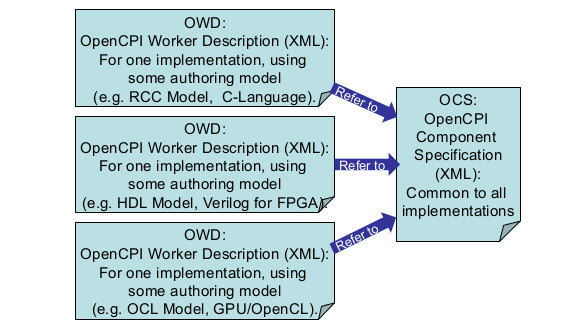
\includegraphics{./figures/owdtoocs.jpg}
\caption{Relationship between \textit{OCS} and \textit{OWD}s}
\label{fig:relations}
\end{center}
\end{figure}
\end{minipage}

\item[Configuration Properties]
\subitem See also \textit{configuration property accessibility}.

Named values of a \textit{worker} that may be read or written by \textit{control software}.
Their values indicate or control aspects of the \textit{worker}'s operation.
Reading and writing these property values may or may not have side effects on the operation of the \textit{worker}.
Configuration properties with side effects can be used for custom worker control.
Each \textit{worker} may have its own, possibly unique, set of configuration properties.
They may include hardware resources such registers, memory, and state.

\item[Configuration Property Accessibility]
Declarations within an \textit{OCS} or \textit{OWD} that indicate \textbf{when} it is valid to read from or write to a \textit{configuration property}.
The various accessibility attributes (defined in the \textit{Component Development Guide}) establish the rules in relation to the \textit{worker}'s \textit{lifecycle} or declare the property as fixed at build-time (see \textit{Parameter}).

\item[Containers]
OpenCPI infrastructure element that ``contains,'' manages, and executes a set of application \textit{workers}. Logically, the container ``surrounds'' the workers, mediating all interactions between the \textit{workers} and the rest of the system.

\item[Control Operations]
A fixed set of control operations that every \textit{worker} has. The control aspect is a common control model that allows all workers to be managed without having to customize the management infrastructure software for each worker, while \textit{configuration properties} are used to specialize components.

\item[Control Plane]
Control and configuration interfaces for runtime \textit{lifecycle} control and configuration of \textit{worker} instances at runtime.

\item[Control Software (AKA Control Application AKA Control Agent)]
The entity that is exercising control using the \textit{ACI}. Encompasses the various aspects of how \textit{control software}, usually running in a centralized host processing environment, can control \textit{worker} instances at runtime via the \textit{control plane}.

\item[Core]
The \textit{project} containing the default \textit{workers} and infrastructure VHDL for the framework to operate.

\item[Data Plane]
Data passing interfaces used for \textit{workers} to consume/produce data from/to other workers in the \textit{application} (of whatever \textit{authoring model} in whatever \textit{container}).

\item[Device Proxy]
A device proxy is a software \textit{worker} (RCC/C++) that is specifically paired with a \textit{device worker} in order to translate a higher level control interface for a class of devices into the lower level actions required on a specific device.

\item[Device Worker]
Special \textit{worker} used for controlling hardware physically attached to an FPGA, \textit{e.g.} a status LED.

\item[Hardware Description Language]
Refers to a specialized language used to program the structure design and operation of digital logic circuits. In OpenCPI, it is an \textit{authoring model} using the VHDL language and is targeted at FPGAs. HDL \textit{workers} should be developed according to the \textit{HDL authoring model} and which is described in the ``OpenCPI HDL Development Guide.''

\item[HDL Assembly]
A fixed composition of HDL \textit{workers} that can act as subset of a heterogeneous OpenCPI \textit{application}.

\item[HDL Assembly Description (OHAD)]
The XML file that describes an \textit{HDL assembly}.

\item[HDL Authoring Model]
The \textit{authoring model} used by the HDL (VHDL-language) \textit{workers}.

\item[Infrastructure]
Software/gateware is either \textit{application} or infrastructure.

\item[isim]
The HDL simulator that Xilinx provides with their ISE software.

% \item[Kernel]
% A function declared in a program and executed on an OpenCL device.

\item[Lifecycle Model]
\begin{minipage}{\textwidth}
The control states each \textit{worker} may be in and \textit{control operations} which generally change the state a worker is in, effecting a state transition:\\
\begin{figure}[H]
\begin{center}
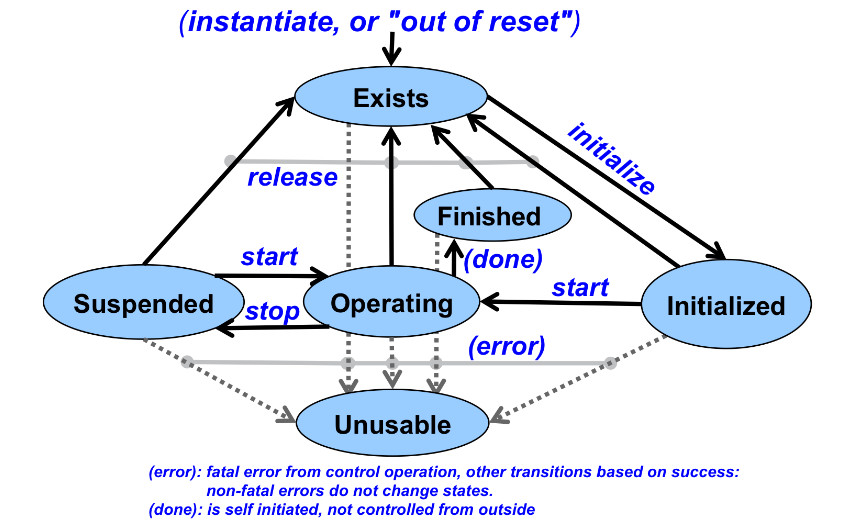
\includegraphics[scale=0.5]{./figures/controlops.jpg}
\caption{The OpenCPI lifecycle model of \textbf{all} \textit{workers}}
\label{fig:lifecycle}
\end{center}
\end{figure}
\end{minipage}

\item[Library]
A conceptually-related set of \textit{components} within a single location (often a \textit{project}).

% \item[OCL Authoring Model]
% \textit{Authoring model} used by the OpenCL language workers.

\item[OpCode]
See \textit{operation code}.

\item[Operation Argument]
Payload data within a \textit{protocol specification} whose type information is determined by the \textit{operation code}.

\item[Operation Code]
Message type encapsulating zero or more \textit{operation arguments} within a \textit{protocol specification}.

\item[Parameter]
An immutable \textit{configuration property} that is set at build time, allowing software compilers and hardware compilers to optimize accordingly.

\item[PCI (Peripheral Component Interconnect)]
Industry-standard local computer bus for attaching hardware devices.

\item[Port Readiness]
Indicates a \textit{worker} has data available, input or output, that the \textit{container} needs to act on. Input ports have available buffers when there is message data present that has not yet been consumed by the \textit{worker}. Output ports are ready when buffers are available into which they may place new data.

\item[Platform]
A particular type of processing hardware and/or software that can host a \textit{container} for executing OpenCPI \textit{workers}.

\item[Platform Configuration]
The XML file that describes a unique configuration of a \textit{platform}.

\item[Platform Worker]
A singleton \textit{worker} that bootstraps the \textit{platform} and \textit{container}.

\item[Primitive]
HDL assets that are lower level than \textit{workers} and may be used (and reused) as building blocks for HDL \textit{workers}.

\item[Project]
Work area in which to develop OpenCPI \textit{components}, \textit{libraries}, \textit{applications}, and other platform- and device-oriented assets.

\item[Project Registry]
A directory that contains references to \textit{projects} in a development environment so they can be referenced by any \textit{project} using that same \textit{project registry}.

\item[Property]
See \textit{Configuration Properties}.

\item[Protocol Specification (OPS)]
One or more XML files that describe the allowable data messages (\textit{operation codes)} and payloads (\textit{operation arguments}) that may flow between the ports of \textit{components}.

\item[Protocol Summary]
The set of all summary attributes, whether inferred from the messages specified for the \textit{protocol}, or specified directly as attributes of the protocol. Indicates the basic behavior of a port using a protocol.  Can also be present when messages are specified, and can override the attributes inferred from the message specifications.

\item[RCC Authoring Model]
\textit{Authoring model} used by the C or C++ language \textit{workers} that execute on general purposes processors (GPPs). The ``Resource Constrained'' prefix indicates the limited set of library calls a worker should use; see the ``OpenCPI RCC Development Guide'' for more information.

\item[Registry]
See \textit{Project Registry}.

\item[Run Condition]
When a \textit{worker} has a combination of \textit{port readiness} and/or some amount of time has passed. Determined by the worker's \textit{container}.

\item[Run Method]
Non-blocking software method that is executed when a \textit{worker}'s \textit{run condition} is satisfied.

\item[Spec file]
Shorthand notation for \textit{component specification} file.

\item[SpecProperty]
XML elements that add \textit{worker}-specific attributes to the \textit{configuration properties} already defined in the \textit{component spec}.

\item[Worker]
Specific implementation of a \textit{component specification} with the source code written according to an \textit{authoring model}.

\item[Worker Description (OWD)]
The XML file describing the \textit{worker} and references the \textit{component spec} it is implementing. See Figure~\ref{fig:relations}.

% \item[Work-Item]
% One of a collection of parallel executions of a kernel invoked on a device. A work-item is executed by one or more processing elements as part of a work-group executing on a compute unit. A work-item is distinguished from other executions within the collection by its global ID and local ID.

\item[XML]
Standardized markup language that defines a set of rules for encoding documents in a format which is both human- and machine-readable.

\item[xsim] The HDL simulator that Xilinx provides with their Vivado software.

\item[Zero Length Message]
Data payload with no \textit{operation arguments} present when a \textit{protocol specification} allows such an \textit{operation code} with no data fields.
\end{description}
\end{document}
